\documentclass[conference]{IEEEtran}
\usepackage{cite}
\usepackage{amsmath,amssymb,amsfonts}
\usepackage{graphicx}
\usepackage{textcomp}
\usepackage{xcolor}
\usepackage{booktabs}
\usepackage{url}
\usepackage{hyperref}
\usepackage{tikz}
\usetikzlibrary{arrows.meta,positioning,fit,calc}

\definecolor{zhblue}{RGB}{31,119,180}
\definecolor{zhorange}{RGB}{255,127,14}
\definecolor{zhteal}{RGB}{0,140,140}
\definecolor{zhred}{RGB}{214,69,65}
\definecolor{zhgreen}{RGB}{44,160,44}

\begin{document}

\title{Zorba Health: Consent-Aware Voice Healthcare AI with FHIR-Grounded RAG and an MCP Tool Gateway}

\author{}

\maketitle

\begin{abstract}
Voice interfaces can make digital health support more accessible, but healthcare agents can expose private data, miss consent requirements, generate unsupported advice, or use tools without adequate controls.
Prior systems such as Polaris are proprietary and cannot be independently audited, and the Model Context Protocol (MCP) standardizes tool access but does not enforce consent or authorization.
We present Zorba Health, an open-source microservice platform for voice healthcare agents.
It combines a LiveKit voice agent, an MCP gateway for controlled tool access, a FHIR-compatible retrieval-augmented generation (RAG) system with citations, and an append-only audit and consent service.
We evaluate the platform on a released synthetic corpus of 16 patients, 646 filtered FHIR resources, 25 question-answer items, 44 emergency-escalation utterances, and 8 consent scenarios.
In offline retrieval tests, the correct record appeared in the top three results for every query (Recall@3 $= 1.00$).
The phrase-based escalation rule scored a perfect F1 of $1.00$ on exact trigger phrases but only $0.29$ on paraphrases (combined $0.71$), showing that rule-based safety is brittle.
End-to-end (e2e) consent tests confirmed that record access is denied, allowed, and restored correctly as consent is revoked and regranted.
In a live OpenAI RAG evaluation, 17 of 20 answerable questions were answered correctly (accuracy $= 0.85$), every answer carried a citation, all five unanswerable probes were safely refused, and mean latency was $1.67$\,s (p95 $2.43$\,s).
Within this synthetic evaluation scope, the results show that separating voice processing, tool policy, clinical retrieval, and compliance logging yields a practical, auditable healthcare agent architecture.
\end{abstract}

\begin{IEEEkeywords}
Healthcare AI, voice agents, FHIR, retrieval-augmented generation, Model Context Protocol, consent, audit, microservices, Synthea
\end{IEEEkeywords}

\section{Introduction}
Telephone and voice channels remain among the most accessible ways for patients to interact with health services, especially for people who struggle with app-centric portals, small screens, or low digital literacy.
Large language models (LLMs) now make natural spoken dialogue practical, so a voice agent can answer questions about a patient's own medications, allergies, and conditions.
Healthcare, however, is a high-stakes domain: any system that touches clinical records must protect privacy, respect patient consent, keep an audit trail, and avoid presenting invented facts as medical information.
The World Health Organization's guidance on large multi-modal models for health emphasizes exactly these governance, accountability, and escalation requirements~\cite{who2024lmm}.

Previous research leaves three gaps.
First, the most capable voice health systems, such as Polaris~\cite{mukherjee2024polaris}, are proprietary: their safety engineering cannot be inspected, reproduced, or extended by the community.
Second, the Model Context Protocol (MCP)~\cite{mcp2024} standardizes how agents call tools, but it explicitly cannot enforce consent or authorization at the protocol layer; every implementor must design those controls, and MCP security surveys document the resulting threat surface~\cite{hou2025mcplandscape}.
Third, safety studies show that crisis and emergency detection degrades sharply on indirect, paraphrased language~\cite{deng2025psycrisisbench,arnaiz2026crisis}, yet published healthcare agent evaluations rarely stress-test this failure mode or release the data needed to reproduce it.

To address these gaps, we propose Zorba Health, an open-source microservice platform in which a voice agent can only reach clinical data through an MCP gateway that checks typed patient consents and writes append-only audit events before any tool runs.
Retrieval-augmented generation (RAG)~\cite{lewis2020rag} over FHIR-derived patient records supplies grounded, citation-bearing answers.
The objective of this study is to answer one engineering question: how can a voice healthcare assistant be built so that tool use, record retrieval, and AI summarization are consent-gated, auditable, grounded in patient-specific FHIR context, and reproducibly evaluable?
Our contributions are:
(1) an open-source voice healthcare microservice architecture;
(2) a controlled MCP tool gateway that materializes the consent flows the MCP specification leaves to implementors;
(3) a FHIR-compatible RAG pipeline with citations;
(4) a safety, consent, and audit framework;
(5) a reproducible synthetic evaluation package including live RAG, consent-gate, and paraphrase safety tests.

The rest of this paper is organized as follows.
Section~II reviews related work and its limitations.
Section~III presents the proposed method.
Section~IV details data collection.
Section~V presents the experimental setup and results.
Section~VI discusses design implications and limitations.
Section~VII concludes.

\section{Related Work}
Bickmore~\textit{et~al.}~\cite{bickmore2010relational} showed that relational virtual agents can empower low-health-literacy patients, establishing the accessibility motivation for conversational care.
Singhal~\textit{et~al.}~\cite{singhal2023medpalm} and Nori~\textit{et~al.}~\cite{nori2023gpt4medicine} demonstrated that modern LLMs encode substantial clinical knowledge.
Mukherjee~\textit{et~al.}~\cite{mukherjee2024polaris} built Polaris, a safety-focused multi-agent voice constellation validated by more than 1{,}100 U.S.\ licensed nurses; it is the closest system to ours in goals but is proprietary and offers no reproducible evaluation artifacts.

On the data side, Walonoski~\textit{et~al.}~\cite{walonoski2018synthea} introduced Synthea for generating synthetic electronic health records, and HL7 FHIR R4~\cite{hl7fhirr4,mandl2016fhir} standardizes their representation, enabling PHI-free research.
Jiang~\textit{et~al.}~\cite{jiang2025medagentbench} released MedAgentBench, a FHIR-compliant virtual EHR benchmark for medical LLM agents.
For grounding, Lewis~\textit{et~al.}~\cite{lewis2020rag} introduced RAG; Es~\textit{et~al.}~\cite{es2023ragas} and Xiong~\textit{et~al.}~\cite{xiong2024medicalrag} contributed RAG evaluation methods for medicine; Zakka~\textit{et~al.}~\cite{zakka2024almanac} (Almanac) and Kabak~\textit{et~al.}~\cite{kabak2026fhirragmeds} (FHIR-RAG-MEDS) showed that retrieval improves clinical answer quality.
For tool use, Yao~\textit{et~al.}~\cite{yao2023react} (ReAct) and Schick~\textit{et~al.}~\cite{schick2023toolformer} (Toolformer) established tool-calling patterns; Schmidgall~\textit{et~al.}~\cite{schmidgall2024agentclinic} and Arora~\textit{et~al.}~\cite{arora2025healthbench} argue for interactive, realistic evaluation.
Around MCP itself, Shehab~\cite{shehab2025agenticai} and ElSayed~\textit{et~al.}~\cite{elsayed2025mcpai} prototype healthcare MCP compliance layers, while Hou~\textit{et~al.}~\cite{hou2025mcplandscape} systematize MCP security threats.
Deng~\textit{et~al.}~\cite{deng2025psycrisisbench} (PsyCrisisBench) and Arnaiz-Rodriguez~\textit{et~al.}~\cite{arnaiz2026crisis} evaluate crisis detection and find models fail on indirect phrasing.

Across these studies, three limitations persist.
Open, end-to-end voice healthcare systems with enforceable consent do not exist: Polaris is closed, and the MCP healthcare prototypes stop short of a running platform with audit guarantees.
Consent and audit are treated as policy discussion rather than as tested system components; HIPAA~\cite{hipaa1996} and WHO guidance~\cite{who2024lmm} demand both.
Finally, safety evaluations rarely publish paraphrase stress sets, so brittleness like that documented by PsyCrisisBench remains invisible in system papers.
These limitations motivate an open architecture whose consent gating, audit logging, and safety behavior are all directly measurable, which is what Zorba Health provides.

\section{Proposed Method}
A new approach is necessary because none of the systems above combines, in one inspectable platform, the four properties a clinical voice agent needs: mediated tool access, enforceable per-patient consent, append-only auditing, and grounded answers with citations.
Bolting a consent check onto a monolithic agent does not work, because the agent process itself still holds database credentials; the design goal is therefore architectural separation, so that the voice runtime is physically unable to touch clinical data except through a policy-checking gateway.
This directly targets the research problem from Section~I: consent gating, auditability, and grounding become properties of the system topology rather than of prompt engineering.

\subsection{Components}
Zorba Health is a set of cooperating microservices (Fig.~\ref{fig:arch}):
an \textbf{API gateway} that terminates client requests and authentication;
a \textbf{voice-agent service} that runs the LiveKit~\cite{livekitagents} speech pipeline (speech-to-text, LLM dialogue, text-to-speech);
an \textbf{MCP gateway} that exposes every clinical capability as a typed tool and is the only path from the agent to backend services;
an \textbf{audit/consent service} that stores typed consent grants (e.g., \texttt{HEALTH\_RECORD\_ACCESS}, \texttt{THIRD\_PARTY\_MODEL\_PROCESSING}) and append-only audit events;
a \textbf{health-records service} implementing the RAG pipeline;
and \textbf{PostgreSQL with pgvector} for record storage and vector search, with Redis for sessions and RabbitMQ for asynchronous events.

Figure~\ref{fig:arch} shows how these pieces connect.
Reading left to right: a patient speaks over the web or a phone call (blue); the voice agent converts speech to a tool request; the request must cross the MCP gateway (orange), which first consults the audit/consent service (red) and only then forwards the query to the health-records RAG service (green), which searches the pgvector store.
The RAG service reports its own audit events back to the audit service, so every data access is logged twice: once at authorization time and once at retrieval time.

\begin{figure}[!t]
\centering
\resizebox{\columnwidth}{!}{%
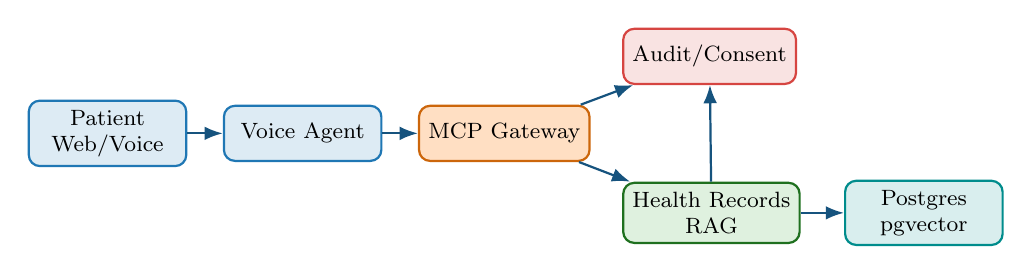
\begin{tikzpicture}[
  font=\footnotesize,
  box/.style={draw, rounded corners, align=center, minimum height=0.7cm, minimum width=2.0cm, thick},
  arr/.style={-{Latex}, thick, zhblue!70!black}
]
\node[box, fill=zhblue!15, draw=zhblue] (pat) {Patient\\Web/Voice};
\node[box, fill=zhblue!15, draw=zhblue, right=0.45cm of pat] (voice) {Voice Agent};
\node[box, fill=zhorange!25, draw=zhorange!80!black, right=0.45cm of voice] (mcp) {MCP Gateway};
\node[box, fill=zhred!15, draw=zhred, above right=0.25cm and 0.4cm of mcp] (audit) {Audit/Consent};
\node[box, fill=zhgreen!15, draw=zhgreen!70!black, below right=0.25cm and 0.4cm of mcp] (hr) {Health Records\\RAG};
\node[box, fill=zhteal!15, draw=zhteal, right=0.55cm of hr] (db) {Postgres\\pgvector};
\draw[arr] (pat) -- (voice);
\draw[arr] (voice) -- (mcp);
\draw[arr] (mcp) -- (audit);
\draw[arr] (mcp) -- (hr);
\draw[arr] (hr) -- (audit);
\draw[arr] (hr) -- (db);
\end{tikzpicture}%
}
\caption{High-level architecture. The voice runtime (blue) can reach clinical data (green/teal) only through the MCP gateway (orange), which checks consent with the audit service (red) first.}
\label{fig:arch}
\end{figure}

Figure~\ref{fig:seq} details one record question as a sequence.
The voice agent issues a tool call (step 1); the MCP gateway asks the audit service whether the patient's \texttt{HEALTH\_RECORD\_ACCESS} consent is active (step 2); if allowed, the gateway forwards the query to the RAG service (step 3), which runs a patient-scoped vector search (step 4) and finally writes an audit event recording what was retrieved (step 5).
If consent is missing at step 2, the call stops there and the denial itself is audited.

\begin{figure}[!t]
\centering
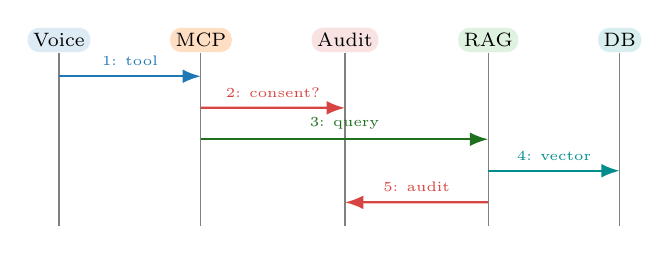
\begin{tikzpicture}[
  font=\scriptsize,
  every node/.style={align=center}
]
\node[fill=zhblue!15, rounded corners, inner sep=2pt] (v) {Voice};
\node[fill=zhorange!25, rounded corners, inner sep=2pt, right=1.0cm of v] (m) {MCP};
\node[fill=zhred!15, rounded corners, inner sep=2pt, right=1.0cm of m] (a) {Audit};
\node[fill=zhgreen!15, rounded corners, inner sep=2pt, right=1.0cm of a] (h) {RAG};
\node[fill=zhteal!15, rounded corners, inner sep=2pt, right=1.0cm of h] (d) {DB};
\foreach \x in {v,m,a,h,d} \draw[gray] (\x.south) -- ++(0,-2.2);
\draw[-{Latex}, thick, zhblue] ([yshift=-0.3cm]v.south) -- node[above]{\tiny 1: tool} ([yshift=-0.3cm]m.south);
\draw[-{Latex}, thick, zhred] ([yshift=-0.7cm]m.south) -- node[above]{\tiny 2: consent?} ([yshift=-0.7cm]a.south);
\draw[-{Latex}, thick, zhgreen!70!black] ([yshift=-1.1cm]m.south) -- node[above]{\tiny 3: query} ([yshift=-1.1cm]h.south);
\draw[-{Latex}, thick, zhteal] ([yshift=-1.5cm]h.south) -- node[above]{\tiny 4: vector} ([yshift=-1.5cm]d.south);
\draw[-{Latex}, thick, zhred] ([yshift=-1.9cm]h.south) -- node[above]{\tiny 5: audit} ([yshift=-1.9cm]a.south);
\end{tikzpicture}
\caption{Sequence of one consent-gated record question (steps 1--5). A missing consent stops the flow at step 2.}
\label{fig:seq}
\end{figure}

\subsection{Consent-Aware RAG}
The RAG pipeline runs six steps: validate the input; check \texttt{HEALTH\_RECORD\_ACCESS}; embed the query; run a vector search restricted to the calling patient's records; optionally summarize using only the retrieved chunks; and emit audit events and citations with the answer.
Restricting search to the patient's own records prevents cross-patient leakage, and returning citations lets a reviewer trace every statement to a source resource.
The present boundary is asymmetric: \texttt{HEALTH\_RECORD\_ACCESS} is enforced before retrieval, but \texttt{THIRD\_PARTY\_MODEL\_PROCESSING} is not yet checked before PHI-derived text is sent to external embedding or chat providers.
The planned gate therefore checks both consent types before any patient-derived text leaves the local trust boundary, denies external processing when the third-party grant is absent, and audits the consent decision, purpose, provider, and outcome.

\subsection{Safety Escalation}
A deterministic phrase classifier scans utterances for emergency language (e.g., chest pain, suicidal intent) and triggers a hospital-visible escalation plus an \texttt{EMERGENCY\_ESCALATION\_TRIGGERED} audit event.
We chose a deterministic rule deliberately as a transparent, high-precision baseline, and Section~V quantifies exactly where it breaks on paraphrases.
Because the current classifier is not deployment-ready for indirect emergency language, the planned mitigation keeps exact-phrase matching as a first high-precision layer, adds a semantic or embedding/LLM detector for paraphrased intent, and escalates or asks a clarifying question when confidence is uncertain.
That hybrid detector must still be evaluated on the released paraphrase set and clinician-reviewed cases before clinical use; it is not claimed as implemented here.

\subsection{Standards Alignment}
Application-level consent types are complementary to the FHIR R4 Consent resource~\cite{hl7fhirconsent}; mapping typed grants to FHIR Consent is future work.
SMART App Launch v2.2 scopes~\cite{smartapplaunch22} authorize FHIR API clients; the MCP gateway sits above SMART-style scopes as a tool-mediation and audit boundary for agent invocations, not as a replacement for OAuth/SMART.

\section{Data Collection}
We construct a synthetic corpus under \texttt{examples/evaluation-data/}; Fig.~\ref{fig:data} shows the construction pipeline.
Reading left to right: Synthea~\cite{walonoski2018synthea} generates patients from a fixed seed; the bundles are slimmed to the FHIR types the platform supports; gold question-answer items and safety/consent scenarios are authored against those records; and the same artifacts feed both offline scoring scripts and the live system evaluation.
Curated gold patients ($n{=}5$) expose explicit facts; Synthea exports ($n{=}10$, seed 1784242671144) add realistic volume; one demo patient completes the set.
Gold QA ($n{=}25$) includes unanswerable LDL-cholesterol probes to test refusal.
Escalation includes exact ($n{=}22$) and paraphrase ($n{=}22$) utterance sets; consent scenarios ($n{=}8$) cover deny, allow, and regrant paths.
Table~\ref{tab:corpus} summarizes resource counts.

\begin{figure}[!t]
\centering
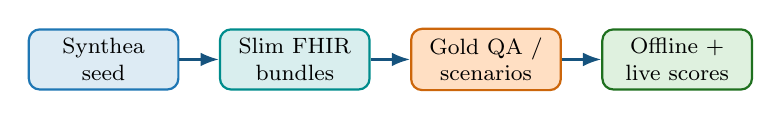
\begin{tikzpicture}[
  font=\footnotesize,
  box/.style={draw, rounded corners, align=center, minimum height=0.65cm, minimum width=1.9cm, thick},
  arr/.style={-{Latex}, thick, zhblue!70!black}
]
\node[box, fill=zhblue!15, draw=zhblue] (syn) {Synthea\\seed};
\node[box, fill=zhteal!15, draw=zhteal, right=0.5cm of syn] (slim) {Slim FHIR\\bundles};
\node[box, fill=zhorange!25, draw=zhorange!80!black, right=0.5cm of slim] (gold) {Gold QA /\\scenarios};
\node[box, fill=zhgreen!15, draw=zhgreen!70!black, right=0.5cm of gold] (score) {Offline +\\live scores};
\draw[arr] (syn) -- (slim);
\draw[arr] (slim) -- (gold);
\draw[arr] (gold) -- (score);
\end{tikzpicture}
\caption{Dataset construction pipeline, from seeded synthetic generation (left) to scored evaluations (right).}
\label{fig:data}
\end{figure}

\begin{table}[!t]
\centering
\caption{Evaluation corpus resource counts (filtered).}
\label{tab:corpus}
\begin{tabular}{@{}lr@{}}
\toprule
Resource type & Count \\
\midrule
Patient & 16 \\
Condition & 126 \\
Observation & 206 \\
MedicationRequest & 97 \\
AllergyIntolerance & 16 \\
Encounter & 80 \\
DiagnosticReport & 60 \\
DocumentReference & 20 \\
CarePlan & 25 \\
\midrule
Total & 646 \\
\bottomrule
\end{tabular}
\end{table}

\section{Experiments and Results}
\subsection{Setup}
The experiments test whether the architecture actually delivers the three properties claimed in Section~I: grounded retrieval, enforced consent, and measurable safety.
All services run locally via Docker Compose; scoring uses Python scripts in \texttt{scripts/evaluation/} and a Go harness (\texttt{eval-live-rag}) that drives the production RAG code path against a local PostgreSQL/pgvector instance and the OpenAI embedding and chat APIs.
We evaluate five things:
(1) \emph{lexical retrieval}: for each gold question, whether the expected resource appears in the top $k{=}3$ type-aware lexical matches (Recall@3);
(2) \emph{live RAG}: the full pipeline under \emph{answer-string-required} scoring, where an answer counts as correct only if the expected fact appears in the answer text itself (a citation alone is not enough);
(3) \emph{consent gating}: an e2e (end-to-end) deny/allow/regrant test that mirrors the pipeline's consent checks and audit statuses;
(4) \emph{safety}: the phrase classifier on exact vs.\ paraphrased emergency utterances;
(5) Go unit and contract tests.
Safety is scored with precision $P$, recall $R$, and
\begin{equation}
F_1 = \frac{2PR}{P + R},
\end{equation}
where a true positive is an emergency utterance that triggers escalation.

\subsection{Results}
Lexical existence and type-aware Recall@3 are both $1.00$: on this corpus, retrieval never fails to surface the right resource, so any answer errors come from generation, not search.
Live RAG answers 17 of 20 answerable questions correctly ($0.85$) with citation presence $1.00$ and safe refusal $1.00$ on the 5 unanswerable LDL probes; mean latency is $1667$\,ms (p95 $2432$\,ms), acceptable for a voice turn.
Error analysis attributes the three misses to allergy facts absent from answer text, plus one answer that incorrectly listed penicillin (an allergy) as a medication --- evidence that generation, not retrieval, is the weak link.

Table~\ref{tab:safety} and Fig.~\ref{fig:safetybars} show the safety stress test.
The phrase classifier is perfect on utterances containing its trigger phrases (F1 $= 1.00$) but recall collapses to $0.17$ on paraphrases (F1 $= 0.29$; combined $0.71$): a patient who says ``my chest feels like it's being squeezed'' instead of ``chest pain'' is missed.
Precision stays $1.00$ throughout --- the rule never over-triggers --- so the failure mode is silence, not noise.
This mirrors the indirect-signal failures reported by PsyCrisisBench~\cite{deng2025psycrisisbench} and Arnaiz-Rodriguez~\textit{et~al.}~\cite{arnaiz2026crisis}, whose LLM-based classifiers reach F1 $\approx 0.88$ on explicit ideation; upgrading from phrase rules to LLM or embedding classifiers is therefore the clear next step, and our released paraphrase set makes that comparison reproducible.
Consent e2e deny/allow/regrant for \texttt{HEALTH\_RECORD\_ACCESS} passes all 11 checks; \texttt{THIRD\_PARTY\_MODEL\_PROCESSING} is not yet gated before external embedding or chat calls and is therefore reported as a known pipeline gap rather than as completed enforcement.

\begin{table}[!t]
\centering
\caption{Emergency escalation: exact vs paraphrase.}
\label{tab:safety}
\begin{tabular}{@{}lrrrr@{}}
\toprule
Split & $n$ & Prec. & Rec. & F1 \\
\midrule
Exact & 22 & 1.00 & 1.00 & 1.00 \\
Paraphrase & 22 & 1.00 & 0.17 & 0.29 \\
Combined & 44 & 1.00 & 0.55 & 0.71 \\
\bottomrule
\end{tabular}
\end{table}

\begin{figure}[!t]
\centering
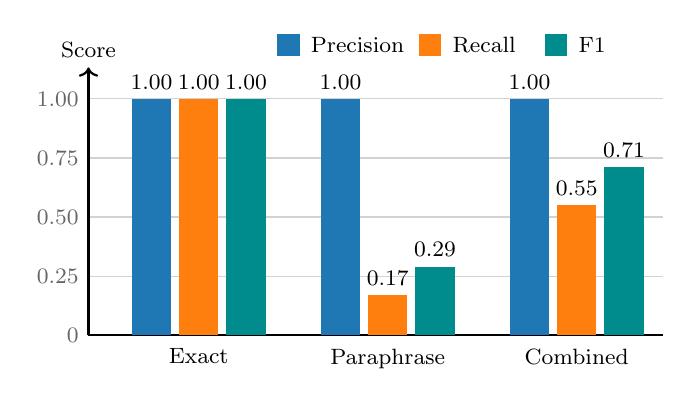
\begin{tikzpicture}[font=\footnotesize]
\def\h{3.0}
% gridlines and y axis
\foreach \y/\lab in {0/0, 0.25/0.25, 0.5/0.50, 0.75/0.75, 1.0/1.00} {
  \draw[gray!35] (0,\y*\h) -- (7.3,\y*\h);
  \node[left, gray!80!black] at (0,\y*\h) {\lab};
}
\draw[->, thick] (0,0) -- (0,3.4) node[above] {Score};
\draw[thick] (0,0) -- (7.3,0);
% bars: precision (blue), recall (orange), F1 (teal)
\foreach \gx/\p/\r/\f/\lbl in {0.55/1.00/1.00/1.00/Exact, 2.95/1.00/0.17/0.29/Paraphrase, 5.35/1.00/0.55/0.71/Combined} {
  \fill[zhblue]   (\gx,0)      rectangle ++(0.5,\p*\h);
  \fill[zhorange] (\gx+0.6,0)  rectangle ++(0.5,\r*\h);
  \fill[zhteal]   (\gx+1.2,0)  rectangle ++(0.5,\f*\h);
  \node[above] at (\gx+0.25,\p*\h) {\p};
  \node[above] at (\gx+0.85,\r*\h) {\r};
  \node[above] at (\gx+1.45,\f*\h) {\f};
  \node[below] at (\gx+0.85,-0.05) {\lbl};
}
% legend
\fill[zhblue]   (2.4,3.55) rectangle ++(0.28,0.28); \node[right] at (2.7,3.69) {Precision};
\fill[zhorange] (4.2,3.55) rectangle ++(0.28,0.28); \node[right] at (4.5,3.69) {Recall};
\fill[zhteal]   (5.8,3.55) rectangle ++(0.28,0.28); \node[right] at (6.1,3.69) {F1};
\end{tikzpicture}
\caption{Emergency-escalation performance by split. Precision is always $1.00$; recall (orange) collapses on paraphrases, dragging F1 (teal) from $1.00$ to $0.29$.}
\label{fig:safetybars}
\end{figure}

\section{Discussion and Limitations}
Separating MCP and audit from the voice runtime creates a single policy enforcement point.
Relative to Hou~\textit{et~al.}~\cite{hou2025mcplandscape}, the gateway mitigates unauthorized tool invocation, weak accountability, and unmediated PHI access, but does not yet address installer spoofing or cryptographic tool-manifest signing.
Relative to Polaris~\cite{mukherjee2024polaris}, we trade proprietary constellation training for an auditable open architecture.

The reported metrics validate engineering behavior on a released synthetic FHIR corpus; they do \emph{not} establish clinical efficacy, real-world crisis safety, or generalization to production electronic health records.
Synthetic FHIR under-represents messy clinical narratives, the live-RAG gold set is modest ($n{=}25$ QA items), and locally measured latency understates telephony round trips.
A staged external-validation path is therefore required: MedAgentBench-style interactive tasks~\cite{jiang2025medagentbench}, clinician-rated groundedness and safety review, and only then governed evaluation on de-identified or real clinical data under IRB and privacy approval.

Three prioritized camera-ready limitations follow directly from the reviews.
First, the phrase-based escalator remains high-precision but low-recall on paraphrases (F1 $0.29$), so a hybrid exact-phrase plus semantic/LLM detector with fail-safe clarification must be evaluated before deployment~\cite{deng2025psycrisisbench,arnaiz2026crisis}.
Second, \texttt{THIRD\_PARTY\_MODEL\_PROCESSING} is not yet enforced before external embedding or chat calls; the next implementation milestone is a deny-by-default gate with audited purpose, provider, and outcome.
Third, typed consents should be mapped to FHIR Consent~\cite{hl7fhirconsent} and composed with SMART scopes~\cite{smartapplaunch22} for EHR interoperability.

\section{Conclusion}
This paper asked how a voice healthcare assistant can be engineered so that tool use, record retrieval, and AI summarization are consent-gated, auditable, grounded in patient-specific FHIR context, and reproducibly evaluable.
Zorba Health answers with architecture rather than prompts: an open-source microservice platform in which an MCP gateway and an append-only audit/consent service stand between the voice agent and all clinical data, and a FHIR-grounded RAG pipeline returns cited answers.
On the released synthetic corpus, retrieval is perfect (Recall@3 $= 1.00$), live RAG reaches $0.85$ answer accuracy with full citation coverage and safe refusals, and consent deny/allow/regrant for health-record access is enforced end-to-end.
An honest paraphrase stress test also exposes the current limit of rule-based escalation (F1 $1.00 \rightarrow 0.29$), and third-party model consent remains an open enforcement gap before external LLM providers.
Within this synthetic scope, the identified problem --- uncontrolled, unauditable agent access to clinical context --- is addressable with system topology, and the open evaluation package lets others verify or beat these numbers.
Future work prioritizes hybrid paraphrase-robust escalation, third-party consent gates inside RAG, FHIR Consent / SMART alignment, MedAgentBench- and HealthBench-style interactive evaluation, clinician review, and governed studies beyond synthetic data.

\section*{Data Availability}
Evaluation artifacts and scripts are included in the open-source repository under \texttt{examples/evaluation-data/} and \texttt{scripts/evaluation/}.
Synthea seed: 1784242671144.
Draft freeze commit: \texttt{2d7429d0}.

\section*{Ethics}
Evaluation uses synthetic data only. No human subjects or production PHI were used. Outputs are not clinical advice.
Framing follows WHO guidance on large multi-modal models for health~\cite{who2024lmm}.

\bibliographystyle{IEEEtran}
\bibliography{refs}

\end{document}
